\chapter{天然物种与合成物种}\label{ch:g10:chemical-species}

一勺香草冰淇淋。它的香味可能来自热带兰花的黑色豆荚，
经采摘、发酵，再在乙醇中浸泡数月；或
也可能来自一家以木浆或
石油为原料制造香精的工厂。并排品尝两者，主要风味相同——
原因很充分：具有香草味的\omterm{def:g7:atoms-and-molecules:molecule}{分子}香草醛，
无论以何种方式获得，它都是完全相同的\omterm{def:g7:atoms-and-molecules:molecule}{分子}。本章将说明
化学家如何从植物中\omterm{def:g10:chemical-species:extraction}{提取}物种、如何制备它，以及
如何核实手中之物确为他们所认定的那种。

\begin{recall}
\omterm{def:g6:pure-substances-and-mixtures:species}{化学物种}是一种特定的物质；\omterm{def:g6:pure-substances-and-mixtures:pure-substance}{纯净物}
只含一种物种，并具有固定的常数，例如其熔点与
沸点（见\cref{ch:g6:pure-substances-and-mixtures}）。液体
可互溶，也可不互溶，每种\omterm{def:g6:solutions-and-solubility:solute}{溶质}
在每种\omterm{def:g6:solutions-and-solubility:solute}{溶剂}中都有其自身的\omterm{def:g6:solutions-and-solubility:solubility}{溶解度}（见\cref{ch:g6:solutions-and-solubility}）。
\omterm{def:g7:identifying-substances:chromatography}{纸色谱法}可分离\omterm{def:g6:pure-substances-and-mixtures:mixture}{混合物}中的染料
（见\cref{ch:g7:identifying-substances}）。
\end{recall}

\begin{omfigure}
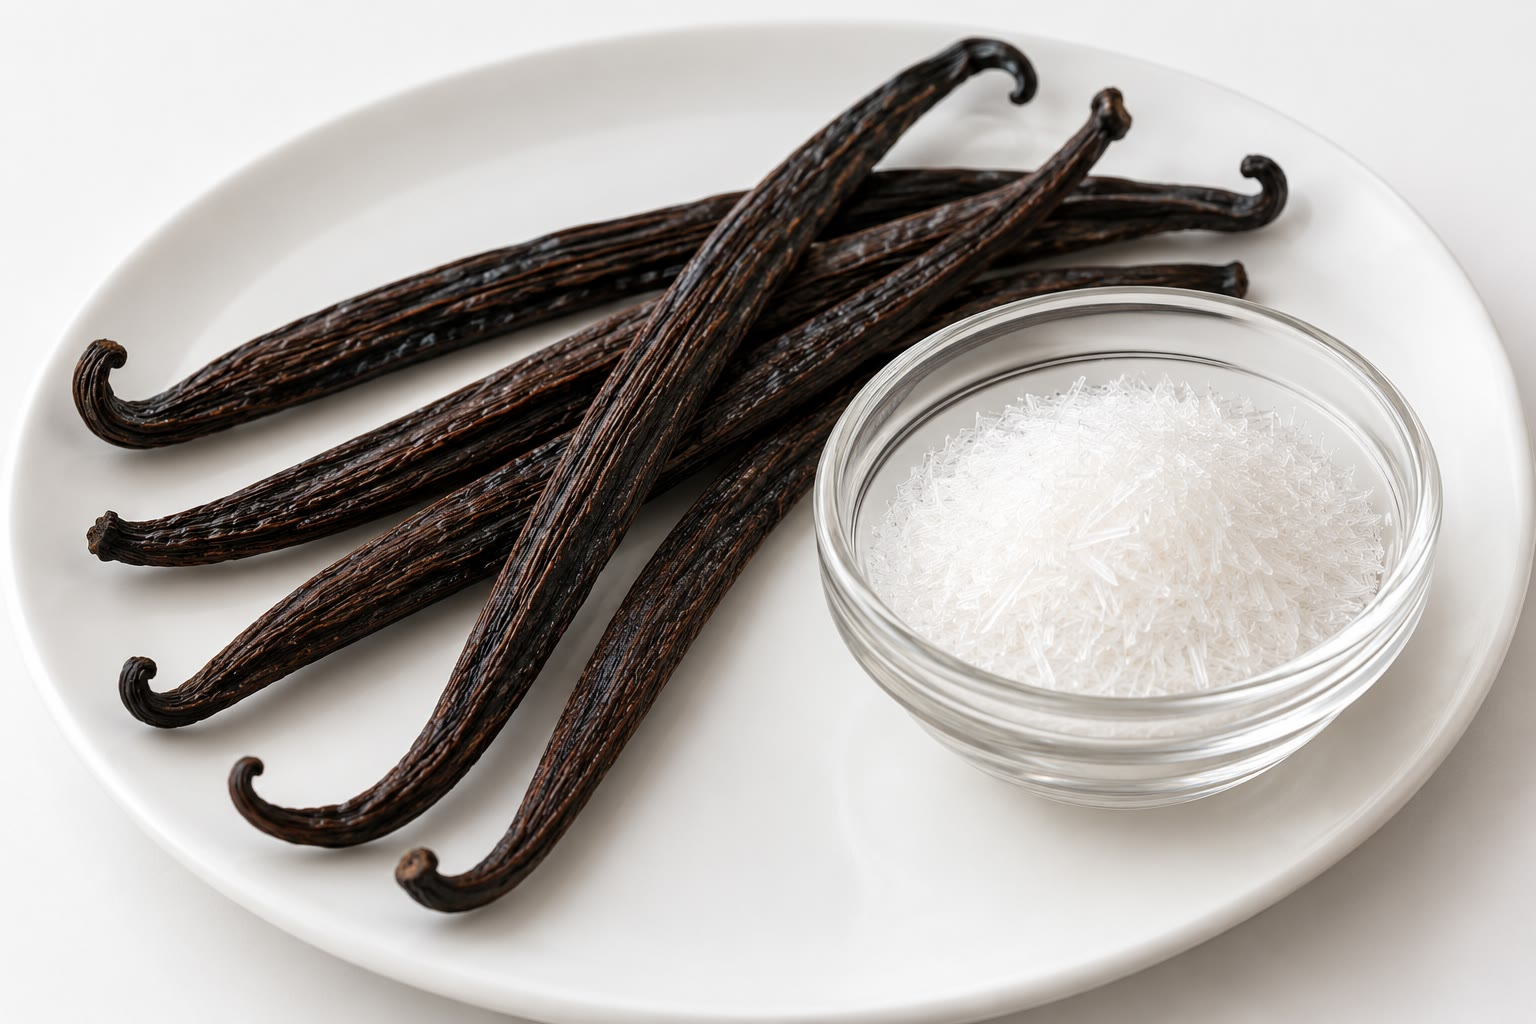
\includegraphics[width=0.55\linewidth]{images/book1/ai/g10-vanilla.jpg}

{\small 香草豆荚与香草醛的白色晶体：同一种\omterm{def:g7:atoms-and-molecules:molecule}{分子}，
来自植物，也可来自工厂。}
\end{omfigure}

\section{天然物种与合成物种}

\begin{definition}[天然物种与合成物种]\label{def:g10:chemical-species:natural}
称\emph{天然物种}\index{天然物种}为由生物制造或在自然界中以此形式存在的
\omterm{def:g6:pure-substances-and-mixtures:species}{化学物种}。称\emph{合成物种}\index{合成物种}为由化学家以
其他物种经
\omterm{def:g7:chemical-reactions:reaction}{化学反应}制成的\omterm{def:g6:pure-substances-and-mixtures:species}{化学物种}。合成物种可与某一天然物种
完全相同（如合成香草醛），
或在自然界中没有对应物（如大多数药物和\omterm{def:g8:plastics:plastic}{塑料}）。
\end{definition}

\begin{proposition}[同一物种，性质相同]\label{prop:g10:chemical-species:same}
无论来源如何，同一\omterm{def:g6:pure-substances-and-mixtures:species}{化学物种}具有相同的性质：
工厂制得的香草醛与从豆荚中\omterm{def:g10:chemical-species:extraction}{提取}的香草醛
具有相同的化学式、相同的熔点与相同的气味。可能不同的
是随之而来的其他成分：天然\omterm{def:g10:chemical-species:extraction}{提取}物是\omterm{def:g6:pure-substances-and-mixtures:mixture}{混合物}，含有许多
会改变其风味的其他物种。
\end{proposition}

\begin{history}[从柳树皮到阿司匹林，1828--1899]
数百年来，人们咀嚼柳树皮以退热止痛。1828 年，一位
化学家从中\omterm{def:g10:chemical-species:extraction}{提取}出有效物种水杨苷；随后，化学家
将其转化为水杨酸，药效虽好却会刺激胃部。
1897 年，费利克斯·霍夫曼在一家染料与制药公司
以水杨酸为原料，制得了更温和的\omterm{def:g10:chemical-species:natural}{合成物种}：乙酰水杨酸，1899 年起
以阿司匹林之名出售。阿司匹林没有天然来源，是纯粹的\omterm{def:g10:chemical-species:natural}{合成物种}。
\end{history}

\section{物种的提取}

\begin{definition}[提取与液–液萃取]\label{def:g10:chemical-species:extraction}
称\emph{提取}\index{提取}为将\omterm{def:g6:pure-substances-and-mixtures:species}{化学物种}从含有它的材料中取出的操作，
通常是将其\omterm{def:g2:mixing-and-dissolving:dissolve}{溶解}于一种选定的\omterm{def:g6:solutions-and-solubility:solute}{溶剂}中。
在\emph{液–液萃取}\index{液–液萃取}中，溶于一种液体的\omterm{def:g6:pure-substances-and-mixtures:species}{化学物种}
被转移到另一种与之不互溶、且在其中\omterm{def:g2:mixing-and-dissolving:dissolve}{溶解}性更好的液体中；
随后，两种液体在
分液漏斗中分离。
\end{definition}

\begin{example}[日常生活中的提取]\label{ex:g10:chemical-species:everyday}
泡茶是用热水进行的\omterm{def:g10:chemical-species:extraction}{提取}（浸泡法）；将香草豆荚
浸泡于乙醇中是用乙醇进行的\omterm{def:g10:chemical-species:extraction}{提取}（浸渍法）；煮
蔬菜熬制高汤则是另一种（煎煮法）。
\end{example}


\begin{definition}[蒸馏与水蒸气蒸馏]\label{def:g10:chemical-species:distillation}
称\emph{蒸馏}\index{蒸馏}为将液体\omterm{def:g6:pure-substances-and-mixtures:mixture}{混合物}加热至沸腾，
使蒸气在由流动的水冷却的冷凝器中重新变为液体，
并收集这种液体，即馏出液。称
\emph{水蒸气蒸馏}\index{水蒸气蒸馏}为将植物材料与水一同煮沸：
水蒸气带走植物中的芳香物种，
这些物种在馏出液中以油层形式与水分离，
即精油。
\end{definition}

\begin{omfigure}
\begin{tikzpicture}[font=\small, scale=0.95]
  \pic[transform shape] at (0,0) {heatingmantle};
  \pic[transform shape] at (0,0) {rbflask={0.55}{omWater!70}};
  \foreach \x/\y in {-0.45/0.35,-0.1/0.55,0.3/0.3,0.5/0.7,-0.6/0.75,0.1/0.9,-0.25/0.2}
    \fill[green!45!black!70] (\x,\y) ellipse (0.09 and 0.04);
  \pic[transform shape] (s) at (0,3.0) {stillhead};
  \pic[transform shape] at ($(s-top)+(0,-0.75)$) {thermometer};
  \pic[transform shape, rotate=-20] (c) at (s-arm) {liebig={3.2}};
  \coordinate (cend) at ($(s-arm)+(-20:3.2)$);
  \pic[transform shape] (a) at (cend) {adapter};
  \pic[transform shape] at ($(a-tip)+(0,-2.3)$) {erlenmeyer={0.18}{omWater!70}};
  \fill[yellow!60!orange!60] ($(a-tip)+(-0.827,-2.3+0.47)$) -- ($(a-tip)+(0.827,-2.3+0.47)$) -- ($(a-tip)+(0.779,-2.3+0.6)$) -- ($(a-tip)+(-0.779,-2.3+0.6)$) -- cycle;
  \draw[<-, omProp, thick] (-0.55,0.55) -- (-2.2,0.9) node[left, text=black, align=right]
    {水和 \\ 薰衣草花};
  \draw[<-, omProp, thick] (1.35,-0.6) -- (2.2,-1.1) node[right, text=black]
    {电热套};
  \draw[<-, omProp, thick] (0.1,4.2) -- (-1.2,4.6) node[left, text=black] {温度计};
  \draw[<-, omProp, thick] ($(s-arm)+(-20:1.6)+(0,0.32)$) -- ++(0.6,1.0) node[above, text=black]
    {冷凝器，经流动的水冷却};
  \draw[<-, omProp, thick] ($(a-tip)+(0.4,-1.88)$) -- ++(1.1,0.2) node[right, text=black, align=left]
    {馏出液：精油 \\ 漂浮在水面上};
\end{tikzpicture}

{\small 薰衣草的\omterm{def:g10:chemical-species:distillation}{水蒸气蒸馏}。水蒸气将精油
带入冷凝器；馏出液分离为
浮在水面上的一薄层油。}
\end{omfigure}

\begin{method}[选择萃取溶剂]\label{met:g10:chemical-species:solvent}
从水中对某物种进行\omterm{def:g10:chemical-species:extraction}{液–液萃取}时，\omterm{def:g6:solutions-and-solubility:solute}{溶剂}必须满足：
必须满足：
\begin{enumerate}
  \item 对该物种的\omterm{def:g2:mixing-and-dissolving:dissolve}{溶解}能力远强于水；
  \item 与水互不相溶，从而形成两层；
  \item 危害尽可能小，且便于事后除去
        （沸点较低，便于其\omterm{def:g3:separating-mixtures:evaporate}{蒸发}）。
\end{enumerate}
哪一层在上，由密度决定：
密度较小的液体漂浮在上层。
\end{method}

\begin{example}[薰衣草精油的溶剂]\label{ex:g10:chemical-species:table}
% ledger: rho:cyclohexane, bp:cyclohexane, rho:ethyl-acetate, bp:ethyl-acetate, rho:CH2Cl2, bp:CH2Cl2, rho:ethanol, bp:ethanol, sol:linalool
芳樟醇是薰衣草精油的主要成分，在水中仅能
\omterm{def:g2:mixing-and-dissolving:dissolve}{溶解} \qty{1.6}{g/L}，但在下列\omterm{def:g6:solutions-and-solubility:solute}{溶剂}中\omterm{def:g2:mixing-and-dissolving:dissolve}{溶解}得很好：
\begin{center}
\small
\begin{tabular}{lccll}
\hline
\omterm{def:g6:solutions-and-solubility:solute}{溶剂} & \qty{1}{mL} 的质量 & 沸点 & 与水的关系 & 主要危害 \\
\hline
环己烷 & \qty{0.78}{g} & \qty{81}{\celsius} & 不互溶 & 易燃、有害 \\
乙酸乙酯 & \qty{0.90}{g} & \qty{77}{\celsius} & 不互溶 & 易燃、刺激性 \\
二氯甲烷 & \qty{1.33}{g} & \qty{40}{\celsius} & 不互溶 & 疑似致癌物 \\
乙醇 & \qty{0.79}{g} & \qty{78}{\celsius} & 互溶 & 易燃 \\
\hline
\end{tabular}
\end{center}
乙醇不能使用，因为它与水混溶，不会分层。
使用环己烷或乙酸乙酯时，\omterm{def:g6:solutions-and-solubility:solute}{溶剂}层在上层；
使用二氯甲烷时，则在下层。
\end{example}

\begin{omfigure}
\begin{tikzpicture}[font=\small, scale=1.2]
  \pic[transform shape] at (0,0) {sepfunnel={omWater!70}{yellow!35!orange!35}};
  \draw[<-, omProp, thick] (0.55,2.1) -- (1.6,2.4) node[right, text=black, align=left]
    {环己烷与精油 \\ （密度较小，在上层）};
  \draw[<-, omProp, thick] (0.55,1.3) -- (1.6,1.2) node[right, text=black, align=left]
    {水，经活塞 \\ 放出};
  \draw[<-, omProp, thick] (0.25,0.52) -- (1.6,0.4) node[right, text=black] {活塞};
\end{tikzpicture}

{\small 振荡并静置后的分液漏斗：精油已
转入上层的环己烷中。}
\end{omfigure}

\begin{safety}{\ghs[0.8cm]{GHS02}\ghs[0.8cm]{GHS07}\ghs[0.8cm]{GHS08}\ghs[0.8cm]{GHS09}}
% ledger: ghs:cyclohexane
环己烷：高度易燃（GHS02）；吞下并进入气道可能致命，
引起皮肤刺激、困倦（GHS07、GHS08）；
对水生生物毒性极大（GHS09）。应在通风橱中使用，
远离明火。
\end{safety}

\section{薄层色谱法}

\begin{definition}[薄层色谱法]\label{def:g10:chemical-species:tlc}
\emph{薄层色谱法}\index{薄层色谱法}（TLC）
是利用涂有一薄层细白粉末的薄板，分离\omterm{def:g6:pure-substances-and-mixtures:mixture}{混合物}中
各物种的方法，该细白粉末称为\emph{固定相}\index{固定相}。
在靠近底部的铅笔线上点上样品的小斑点；
将薄板置于密闭的槽中，槽内加有少量\omterm{def:g6:solutions-and-solubility:solute}{溶剂}，
即\emph{洗脱剂}\index{洗脱剂}，它沿薄板上升，
将各物种带到取决于该物种的高度。无色斑点
随后在紫外线下或借助碘蒸气使其显现。
\end{definition}

\begin{definition}[比移值]\label{def:g10:chemical-species:retention-factor}
某斑点的\emph{比移值}\index{比移值}为
\[
  R_f = \frac{\text{从起始线到斑点的距离}}
             {\text{从起始线到溶剂前沿的距离}},
\]
它是介于 0 与 1 之间的一个数。在给定的薄板、\omterm{def:g10:chemical-species:tlc}{洗脱剂}和温度下，
每种物种都有各自的 $R_f$。
\end{definition}

\begin{method}[薄层色谱的操作与读数]\label{met:g10:chemical-species:tlc}
\begin{enumerate}
  \item 用铅笔在距底部 \qty{1}{cm} 处画出起始线；
        在起始线上为每个样品和每种参照物种
        各点一个小斑点。
  \item 将薄板放入槽中，\omterm{def:g10:chemical-species:tlc}{洗脱剂}位于起始线之下；
        盖紧槽体。
  \item \omterm{def:g6:solutions-and-solubility:solute}{溶剂}前沿距顶部约 \qty{1}{cm} 时，取出薄板；
        立即标出前沿位置，晾干并显色。
  \item 测量各距离，并计算每个斑点的 $R_f$。若某样品
        只出现一个斑点，则很可能是\omterm{def:g6:pure-substances-and-mixtures:pure-substance}{纯净物}种；
        若斑点与同一薄板上某参照斑点高度相同，
        则很可能就是该物种。
\end{enumerate}
\end{method}

\begin{omfigure}
\begin{tikzpicture}[font=\small, scale=1.25]
  % the tank
  \pic[transform shape] at (0,0) {beaker={0.15}{omWater!80}};
  \fill[white] (-0.55,0.08) rectangle (0.55,1.92);
  \fill[omWater!80] (-0.55,0.08) rectangle (0.55,0.3);
  \draw[omGlass, line width=0.6pt] (-0.55,0.08) rectangle (0.55,1.92);
  \draw[black!60] (-0.55,0.42) -- (0.55,0.42);
  \foreach \x in {-0.3,0,0.3} \fill[black!70] (\x,0.42) circle (0.04);
  \fill[black!25] (-1.0,2.08) rectangle (1.0,2.18);
  \node[anchor=north, align=center] at (0,-0.15) {密闭的槽 \\ 加盖};
  % the developed plate
  \begin{scope}[xshift=4.2cm]
    \pic[transform shape] at (0,0) {tlcplate};
    \draw[black!50, dashed] (-0.7,2.8) -- (0.7,2.8);
    \fill[omDef!70] (-0.35,1.36) ellipse (0.1 and 0.07);
    \fill[omDef!70] (-0.35,2.2) ellipse (0.1 and 0.07);
    \fill[omDef!70] (0,1.36) ellipse (0.1 and 0.07);
    \fill[omDef!70] (0.35,2.2) ellipse (0.1 and 0.07);
    \foreach \x/\l in {-0.35/O,0/L,0.35/A} \node[font=\footnotesize, anchor=north] at (\x,0.38) {\l};
    \draw[<->, omProp] (0.95,0.4) -- (0.95,1.36) node[midway, right, text=black, font=\footnotesize] {$d$};
    \draw[<->, omProp] (1.55,0.4) -- (1.55,2.8) node[midway, right, text=black, font=\footnotesize] {$D$};
    \draw[black!40, densely dotted] (-0.25,1.36) -- (0.95,1.36);
    \node[anchor=north, align=center] at (0.2,-0.15) {显色后的薄板：\\ $R_f = d/D$};
  \end{scope}
\end{tikzpicture}

{\small TLC：薰衣草精油（O）与芳樟醇（L）、乙酸芳樟酯
（A）并列。精油给出两个斑点，高度与两个参照物相同，
说明其中含有两种物种。对芳樟醇而言，$R_f = d/D$。}
\end{omfigure}

\section{通过物理常数识别物种}

\begin{proposition}[熔点可用于检验身份与纯度]\label{prop:g10:chemical-species:mp}
% ledger: mp:vanillin, mp:aspirin, mp:salicylic
纯净固体在自身温度下熔化得很集中：香草醛约在
\qty{82}{\celsius}，阿司匹林在\qty{135}{\celsius}，水杨酸在
\qty{158}{\celsius}。不纯的样品熔化温度更低，且熔化范围
跨越数度。用加热的\omterm{def:g9:periodic-table-first-look:metal}{金属}台或熔点仪测定熔点，因此既能
鉴定固体的身份，也能
判断它是否纯净。
\end{proposition}

\begin{inthelab}[一块 TLC 板]
学生在一块板上点样薰衣草精油、芳樟醇和乙酸芳樟酯，
用教师选定的\omterm{def:g2:mixing-and-dissolving:mix}{混合}\omterm{def:g6:solutions-and-solubility:solute}{溶剂}，在密闭广口瓶中展开，
再在紫外灯下显色，同时戴上能挡住紫外线的护目镜。
\omterm{def:g10:chemical-species:tlc}{洗脱剂}须
在通风橱中取用与处理。
\end{inthelab}

\begin{omfigure}
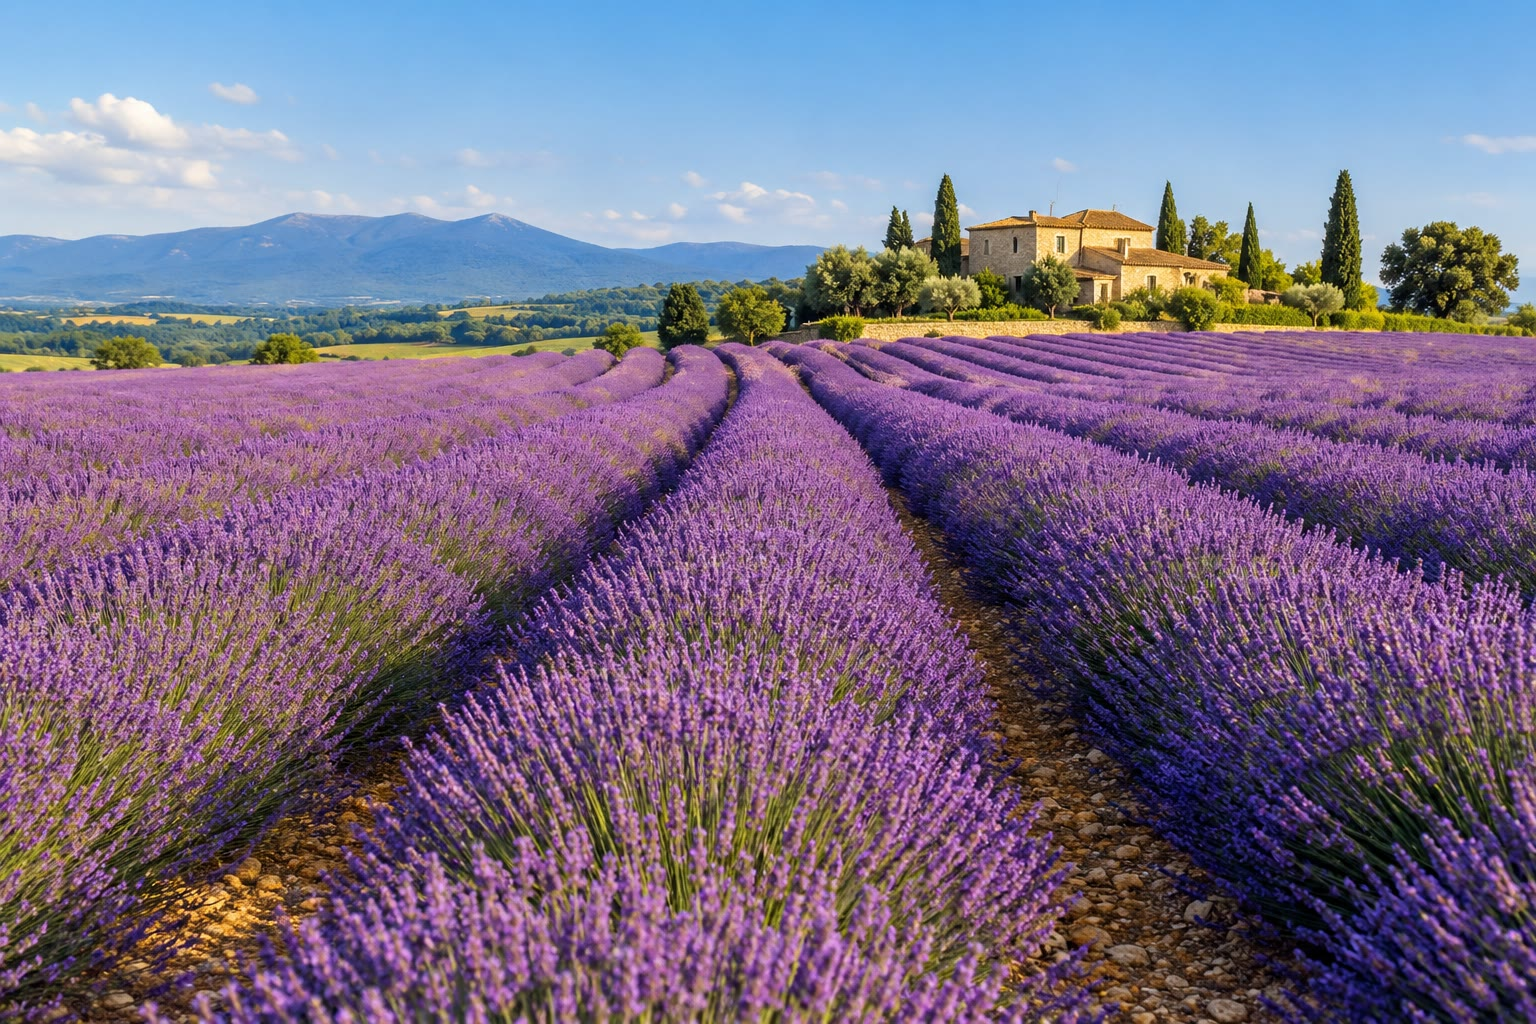
\includegraphics[width=0.55\linewidth]{images/book1/ai/g10-lavender-field.jpg}

{\small 盛花中的薰衣草田：薰衣草
精油的原料。}
\end{omfigure}

\section{练习}

\begin{exercise}[$\star$]\label{exo:g10:chemical-species:1}
判断下列物种是\omterm{def:g10:chemical-species:natural}{天然物种}还是\omterm{def:g10:chemical-species:natural}{合成物种}：香草荚中的香草醛、阿司匹林、
咖啡豆中的咖啡因、工厂制得的香草醛。
\end{exercise}

\begin{exercise}[$\star$]\label{exo:g10:chemical-species:2}
为什么合成香草醛与天然香草醛的
熔点相同？
\end{exercise}

\begin{exercise}[$\star$]\label{exo:g10:chemical-species:3}
在 TLC 板上，\omterm{def:g6:solutions-and-solubility:solute}{溶剂}前沿高出起始线 \qty{6.0}{cm}，
某斑点高出起始线 \qty{2.4}{cm}。求该斑点的 $R_f$。
\end{exercise}

\begin{exercise}[$\star$]\label{exo:g10:chemical-species:4}
说明冷凝器在\omterm{def:g10:chemical-species:distillation}{蒸馏}中的作用，并解释冷水为何
从其下端通入。
\end{exercise}

\begin{exercise}[$\star$]\label{exo:g10:chemical-species:5}
写出萃取\omterm{def:g6:solutions-and-solubility:solute}{溶剂}必须满足的三个条件。
\end{exercise}

\begin{exercise}[$\star\star$]\label{exo:g10:chemical-species:6}
根据\omterm{def:g6:solutions-and-solubility:solute}{溶剂}表，解释为何乙醇不能用于从馏出液中
萃取芳樟醇，而环己烷可以。
\end{exercise}

\begin{exercise}[$\star\star$]\label{exo:g10:chemical-species:7}
在分液漏斗中将二氯甲烷与水\omterm{def:g2:mixing-and-dissolving:mix}{混合}振荡，指出哪一层
位于上层，并结合表中数据说明理由。
\end{exercise}

\begin{exercise}[$\star\star$]\label{exo:g10:chemical-species:8}
一种标称为阿司匹林的白色粉末在 \qty{126}{\celsius} 开始熔化，
在 \qty{132}{\celsius} 时完全熔化。能得出什么结论？
\end{exercise}

\begin{exercise}[$\star\star$]\label{exo:g10:chemical-species:9}
观察本章的 TLC 图，指出薰衣草精油含有哪些物种，
并判断哪种物种上升得更高。
\end{exercise}

\begin{exercise}[$\star\star$]\label{exo:g10:chemical-species:10}
请将实验室获取薰衣草精油的步骤排序：
分离各层；\omterm{def:g10:chemical-species:distillation}{水蒸气蒸馏}；向
馏出液中加入环己烷并振荡；\omterm{def:g3:separating-mixtures:evaporate}{蒸发}环己烷。
\end{exercise}

\begin{exercise}[$\star\star$]\label{exo:g10:chemical-species:11}
为什么 TLC 板的起始线要用铅笔画，并且要位于
\omterm{def:g10:chemical-species:tlc}{洗脱剂}液面之上？
\end{exercise}

\begin{exercise}[$\star\star\star$]\label{exo:g10:chemical-species:12}
萃取后，通过缓慢加热除去环己烷，留下
精油。结合环己烷与芳樟醇（\qty{198}{\celsius}）的沸点，解释
这一操作为何可行。
\end{exercise}

\begin{exercise}[$\star\star\star$]\label{exo:g10:chemical-species:13}
某风味物质样品在 TLC 板上只显示一个斑点，其高度与
\omterm{def:g10:chemical-species:natural}{天然物种}的相同，并且在正确的温度下熔化得很集中。
请指出可以得出的两个结论。
\end{exercise}

\begin{exercise}[$\star\star\star$]\label{exo:g10:chemical-species:14}
在同一张 TLC 板上，斑点 A 的 $R_f = 0.40$，\omterm{def:g6:solutions-and-solubility:solute}{溶剂}前沿高出
起始线 \qty{5.5}{cm}。求斑点 A 的高度。另一物种的
$R_f = 0.75$，求它比斑点 A 高出多少。
\end{exercise}

\begin{exercise}[$\star\star\star$]\label{exo:g10:chemical-species:15}
\qty{1.6}{g} 芳樟醇可\omterm{def:g2:mixing-and-dissolving:dissolve}{溶解}于 \qty{1}{L} 水中。某馏出液
为 \qty{200}{mL} 水，溶有 \qty{0.20}{g} 芳樟醇。该馏出液是否
已饱和？还能再\omterm{def:g2:mixing-and-dissolving:dissolve}{溶解}多少？为何值得用环己烷萃取
这些水，而不是直接弃去？
\end{exercise}

\clearpage % keeps the heading with its problem box (it was stranded at a page foot)
\section{问题：薰衣草的香气}

\begin{problem}[{周末问题——从一篮薰衣草花到
几滴精油，经色谱法检验}]
\label{pb:g10:chemical-species:1}
% ledger: rho:cyclohexane, bp:cyclohexane, rho:CH2Cl2, bp:linalool, ghs:cyclohexane
在学校实验室中，将 \qty{100}{g} 新鲜薰衣草花
与水进行\omterm{def:g10:chemical-species:distillation}{水蒸气蒸馏}。馏出液呈浑浊状，在分液漏斗中与
\qty{20}{mL} 环己烷振荡；保留环己烷层，
将其干燥，再用温和加热的方式\omterm{def:g3:separating-mixtures:evaporate}{蒸发}除去环己烷。剩下的为
薰衣草精油。请使用本章中的
\omterm{def:g6:solutions-and-solubility:solute}{溶剂}表。

\medskip
\noindent\textbf{第一部分——\omterm{def:g10:chemical-species:distillation}{水蒸气蒸馏}。}
\begin{enumerate}
  \item 在\omterm{def:g10:chemical-species:distillation}{水蒸气蒸馏}中，沸腾的水起什么作用？
  \item 冷凝器的作用是什么？冷水从何处
        进入冷凝器？
  \item 馏出液上方可见一层薄薄的油状物漂浮在水面上。该油
        是否与水互溶？它的密度比水大还是小？
  \item 为何不直接倾出馏出液以回收该油？
\end{enumerate}

\medskip
\noindent\textbf{第二部分——萃取。}
\begin{enumerate}[resume]
  \item 为何环己烷适合用作本次萃取的\omterm{def:g6:solutions-and-solubility:solute}{溶剂}？
  \item 能否改用乙醇？请说明理由。
  \item 振荡并\omterm{def:g3:separating-mixtures:decant}{沉降}后，环己烷层位于上层还是下层？
        若改用二氯甲烷，又会如何？
  \item 根据环己烷的象形图，给出两条所需的注意事项。
  \item 为何蒸去环己烷时不会损失
        沸点为 \qty{198}{\celsius} 的芳樟醇？
\end{enumerate}

\medskip
\noindent\textbf{第三部分——色谱法。}
将精油、纯芳樟醇（L）和纯乙酸芳樟酯（A）点样于
一块 TLC 板上。展开后，\omterm{def:g6:solutions-and-solubility:solute}{溶剂}前沿高出 \qty{6.0}{cm}
起始线。精油给出两个斑点，分别位于 \qty{2.4}{cm} 和
\qty{4.5}{cm} 处；斑点 L 位于 \qty{2.4}{cm}，斑点 A 位于 \qty{4.5}{cm}。
\begin{enumerate}[resume]
  \item 计算芳樟醇和乙酸芳樟酯的 $R_f$。
  \item 就本板所示，精油含有什么成分？
  \item 薰衣草精油是\omterm{def:g6:pure-substances-and-mixtures:pure-substance}{纯净物}吗？
  \item 为何要将对照品与精油点在同一块板上？
  \item 将合成芳樟醇点在另一块板上，两者展开条件相同。
        其斑点的 $R_f = 0.40$，可得出什么结论？
\end{enumerate}

\medskip
\noindent\textbf{第四部分——精油有多少？}
所得精油的体积为 \qty{1.0}{mL}；此精油
\qty{1}{mL} 的质量为 \qty{0.90}{g}。
\begin{enumerate}[resume]
  \item 所得精油的质量是多少？
  \item 该质量占花质量的百分之几？
  \item 得到 \qty{100}{g} 精油需要多少质量的花？
  \item 据称该精油是“天然”的。在何种意义上这一说法成立？该精油中的芳樟醇
        是否不同于合成芳樟醇？
  \item 写出由 \qty{100}{g} 花所得
        精油的质量。
\end{enumerate}
\end{problem}
